\chapter{Análisis de requisitos}

\section{Requisitos funcionales y no funcionales}
{\color{red}Creo que lo de detectar letras de forma inmediata debería
ser un requisito funcional, ya que si no es así, el sistema no
funcionaría. Hay alguno más que lo mismo deberías cambar a
funcional, porque son relativos al funcionamiento del sistema. Revisa
los apuntes de IS para no meter la pata aquí o te crucificarán los
de LSI. Los requisitos no funcionales son del tipo "debe funcionar con
baterías", "debe programarse en ADA", "las dimensiones no pueden
pasar de tanto", "No puede pesar más de tanto", etc.}
\subsection{Requisitos funcionales}
\begin{itemize}
    \itemsep0em 
    \item El sistema procesará el movimiento resultando en la
    identificación de una letra.
    \item El sistema enviará la letra identificada por el sistema
    de comunicación pertinente.
    \item Al detectar un movimiento despreciable, el sistema lo descartará.
    \item Posterior a la identificación del movimiento, el sistema
    dejará un periodo suficiente de no registro de movimiento para
    que el usuario recoloque su postura.
    \item El sistema debe contar con una interfaz que medie entre
    el dispositivo y el usuario.
\end{itemize}


\subsection{Requisitos no funcionales}
\begin{itemize}
    \itemsep0em 
    \item El sistema debe funcionar con comunicación por cable e inalámbrica.
    \item El tiempo de procesamiento para la identificación de la letra,
    debe ser inmediato para generar sensación de escritura natural.
    \item La identificación de la letra debe ser eficaz y consistente.
    \item La interfaz de usuario debe ser simple de entender y usar.
    \item El sistema debe contar con autonomía energética.
\end{itemize}


\section{Análisis de requisitos hardware\label{reqHW}}
El dispositivo a crear clasificará, de forma autónoma, los distintos
gestos que se realicen
como letras, usando como herramienta de procesamiento Deep Learning.
Por tanto la placa debe contar con:
\begin{itemize}
    \itemsep0em 
    \item Un módulo que pueda computar tensores.
    \item Sensores suficientes para hacer
    reconocible el movimiento con precisión. En su defecto, se integrarán.
    \item Tecnología bluetooth. En su defecto, se integrará.
    \item Unas dimensiones reducidas.
    \item Documentación para su utilización y el respaldo de una comunidad
    activa para tener otros proyectos como soporte.
\end{itemize}

\section{Planificación y presupuestación}
\subsection{Planificación}
La planificación ha sido esencial para poner en valor los tiempos que manejar
y ser consciente de las limitaciones.
Es lo primero que se debe plantear unido a una preparación o documentación
sobre lo que se va a trabajar para, solo de esta forma, poder estimar de una
forma más precisa los plazos de cada elemento ineludible en el desarrollo
del producto que se busca.
\begin{figure}[]
    \centering
    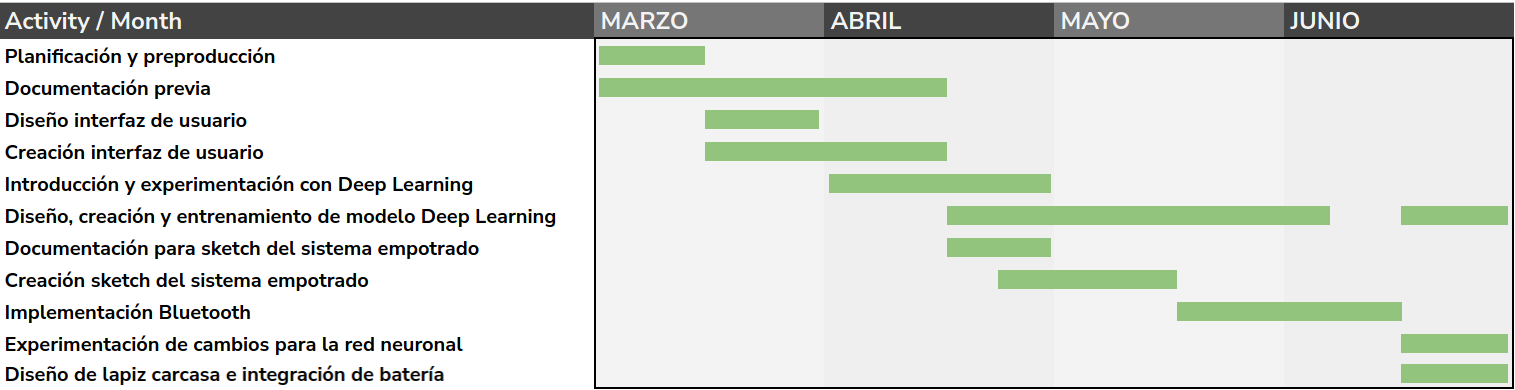
\includegraphics[angle=270,width=0.47\textwidth]{capturas/ganttFixed.png}\\[-0,20cm]
    \caption{Diagrama \textit{Gantt} para la planificación}
\end{figure}

Como muestra la \textit{figura 3.1}, ha sido una planificación basada en contenidos, sin prácticamente iteraciones
de desarrollo, ya que, dados todos los campos que se abarcan
y dada la complejidad de alguno de ellos; es improbable poder
contar con varias iteraciones. La excepción de este precepto viene
con el modelo, con el que se trató de experimentar, con franqueza más
por apetencia de estudiar las redes neuronales y su desempeño, que por
necesidad.

Aunque solo encontramos esa segunda iteración o revisión en la red neuronal,
hay un cierto patrón de documentación y ejecución para cada parte del
proyecto, por lo que se podría decir que los procesos están fraccionados.
Sin embargo no deja de ser, como se ha denominado anteriormente, una
planificación basada en contenidos: se ejecuta una parte y se procede con
la siguiente.
\newpage
El orden ha sido relevante y tiene su propósito. En primer lugar
está la documentación  y planificación, seguida de la creación de
la interfaz, no por otra cosa que la carencia del hardware. Estos plazos
son los primeros ya que permiten trabajar sin el sistema empotrado; tiempos
de selección y obtención del hardware. Complementariamente, el diseño
de la interfaz de usuario abre la mente a reflexionar sobre qué podría
ofrecer el dispositivo a la persona que hace uso de él, ayuda a pensar
en nuevas funcionalidades.

El siguiente bloque de contenido es el del modelo basado en
\textit{Deep Learning}, ya que si el modelo no alcanzara en la fase de
testeo unos resultados óptimos, todavía podemos contar con algo más de
tiempo para solventar su eficiencia.

Y por último la creación del propio sketch y la integración del bluetooth,
dividida en la implementación en la interfaz de usuario y en el programa
gestor del hardware (\textit{sketch}); para poder congregar finalmente
todos los elementos y probar el resultado del producto.

Una última fase de experimentación en la que también se incluirá la creación
y producción del embellecimiento para el dispositivo en forma de lápiz y la
integración de su batería en el mismo.

\subsection{Presupuesto}
Para esta sección ha de tenerse en consideración que el precio de la electrónica
es superior al ordinario debido a la escasez en la producción.

\begin{table}[h]
    \begin{tabular}{ll}
    \hline
    \rowcolor[HTML]{6665CD} 
    \multicolumn{1}{|l|}{\cellcolor[HTML]{6665CD}{\color[HTML]{EFEFEF} \textbf{Descripción}}} & \multicolumn{1}{l|}{\cellcolor[HTML]{6665CD}{\color[HTML]{EFEFEF} \textbf{Precio}}} \\ \hline
    \multicolumn{1}{|l|}{Arduino Nano Sense 33 BLE ~~~~~~~~~~~~~~~~~~~~~~~~~~~~~~~~~~~~~}& \multicolumn{1}{r|}{35'80\$$\sim$33'82€}                                            \\
    \multicolumn{1}{|l|}{Pila 9V Recargable}                                                  & \multicolumn{1}{r|}{10'99€}                                                         \\
    \multicolumn{1}{|l|}{Impresión}                                                           & \multicolumn{1}{r|}{1€}                                                             \\
    \multicolumn{1}{|l|}{Cable MicroUSB Datos}                                                & \multicolumn{1}{r|}{6€}                                                             \\ \hline
    \multicolumn{1}{r}{\textbf{TOTAL:}}                                                       & \textbf{51,81€}                                                                    
    \end{tabular}
    \end{table}